\section{Automatic Distributed Monitoring} \label{sec:method}

We aim to provide an automatic method for distributed monitoring of arbitrary functions of the global aggregate $\bar{x}$.
Given a function specified by a computer program, we automatically generate a communication-efficient scheme to monitor this function.

We first describe ADCD (for \emph{Automatic DC Decomposition}), the automatic local constraint technique that lies at the heart of AutoMon.
ADCD uses automatic differentiation and numerical optimization to derive local constraints for arbitrary functions.
We describe two variants of ADCD, one for general functions (\S\ref{sec:adcd_by_extreme_eigenvalue}) and the other for functions with constant Hessian (\S\ref{sec:adcd_by_eigendecomposition}).
ADCD detects the type of the function and uses the best ADCD variant accordingly to provide a DC decomposition, which it then converts to a GM-style local constraint (\S\ref{sub_sec:adcd}) that can be plugged-in to the GM protocol.
%
We also explore how the type of DC decomposition (convex or concave)  affects the quality of the derived constraints, and propose a heuristic for choosing between convex difference and concave difference (\S\ref{sub_sec:convex_vs_concave_difference}). 

We then describe how AutoMon combines ADCD with the GM protocol to do functional monitoring~(\S\ref{sub_sec:basic-protocol}).
%
Additionally, we consider a novel aspect of the problem: the impact of limiting the monitoring to a small part of the domain in a neighborhood around the reference point, using local constraints that are customized to this neighborhood (\S\ref{sub_sec:sub_domain_size}).
%
Finally, we discuss correctness guarantees (\S\ref{sec:correctness_guarantees}) and implementation considerations (\S\ref{sec:implementation}).


\subsection{ADCD by Extreme Eigenvalue (ADCD-X)} \label{sec:adcd_by_extreme_eigenvalue}

The following lemma shows how to obtain a DC decomposition of a twice differential function $f(x)$.
Recall a function $f$ is convex if and only if its Hessian $H$ is positive semidefinite (denoted $H \succeq 0$), i.e., its smallest eigenvalue is non-negative.
Conversely, $f$ is concave if its largest eigenvalue is non-positive, $H \preceq 0$.
The idea behind the lemma is that $f$ can be ``made convex'' by adding another function such that the Hessian is positive semidefinite (PSD).
The added function must be convex and the difference between the altered function and the added function is the required DC decomposition.
The added function construction is based on the extreme eigenvalues of the Hessian of the function.
Note, the lemma is defined over some set $\FS$, which can be the full domain $\FD$ or a subset of it.

\begin{lemma} \label{lemma:adcd_by_extreme_eigenvalue}
Let $f(x)$ be a twice differentiable function with domain $\FD$, and let $\FS \subseteq \FD$ be a subset of the domain. 
Let $\lambda_{\min}$ and $\lambda_{\max}$ be the smallest and largest eigenvalues of the Hessian $H(x)$ of $f(x)$ where $x\in \FS$,
and define $\lambda^{-}_{\min} \coloneqq \min\{0, \lambda_{\min}\}$ and $\lambda^{+}_{\max} \coloneqq \max\{0, \lambda_{\max}\}$.

Then \eqref{eq:lemma1-convex} is a convex difference of $f(x)$ over $\FS$:
\begin{align}
\label{eq:lemma1-convex}
f(x) = \underbrace{f(x) + \frac{1}{2}\abs{\lambda^-_{\min}} \norm{x-x_0}^2 }_{\text{convex }\check{g}(x)} - \underbrace{\frac{1}{2}\abs{\lambda^-_{\min}} \norm{x-x_0}^2}_{\text{convex }\check{h}(x)}
\end{align}
and \eqref{eq:lemma1-concave} is a concave difference of $f(x)$ over $\FS$:
\begin{align}
\label{eq:lemma1-concave}
f(x) = \underbrace{ f(x) - \frac{1}{2}\lambda^{+}_{\max} \norm{x-x_0}^2 }_{\text{concave }\hat{g}(x)} - \underbrace{\frac{-1}{2}\lambda^{+}_{\max} \norm{x-x_0}^2}_{\text{concave }\hat{h}(x)}.
\end{align}
\end{lemma}


The proof of Lemma~\ref{lemma:adcd_by_extreme_eigenvalue} uses the fact that $\lambda^{-}_{\min} \leq \lambda_{\min}$ to show that Hessians of $\check{g}$ and $\check{h}$ are PSD, which implies $\check{g}$ and $\check{h}$ are convex, and similarly show that $\hat{g}$ and $\hat{h}$ are concave.
The full proof is omitted due to space limitation.


Lemma~\ref{lemma:adcd_by_extreme_eigenvalue} shows how to construct a DC decomposition if we are given the extreme eigenvalues.\footnote{An informal version of \eqref{eq:lemma1-convex} appears in~\cite{lazerson:lightweight_monitoring}, where it is used for manual analysis of specific functions rather than automatically for general function.}
Alas, finding the extreme eigenvalues of a general function, with an $x$-dependent Hessian matrix, is a difficult task~\cite{interval_matrix_branch_and_bound}.
The Hessian $H(x)$ is a function of $x$, and therefore its eigenvalues are a function of $x$.
Finding the $x$ in $\FS$ that obtains the minimal or maximal eigenvalue is not trivial.
Therefore, instead of finding the extreme eigenvalues analytically, we use numerical techniques to solve this problem.


\betterparagraph{Using Automatic Differentiation}
Using Lemma~\ref{lemma:adcd_by_extreme_eigenvalue} requires obtaining $H(x)$ and finding $x',x'' \in \FS$ that obtain $\lambda_{\min}$ and $\lambda_{\max}$.
Our key insight here is that we do not need an analytic solution for $\lambda_{\min}$ and $\lambda_{\max}$, nor a symbolic expression of $H(x)$, but rather a way to evaluate $H$ for specific points in $\FS$.
Since we are given an arbitrary $f(x)$ in the form of a short program, AD enables this automatic evaluation of $H$ in any $x \in \FS$.
By evaluating $H$ using AD at multiple points in $\FS$, and computing the extreme eigenvalues of each such Hessian, we can find the global minimum and maximum $\lambda_{\min}$ and $\lambda_{\max}$.
Instead of evaluating $H$ at random points, we define and solve an optimization problem, which is a more robust and efficient method to find these extreme values.

Another advantage of using AD is that it allows us to apply Lemma~\ref{lemma:adcd_by_extreme_eigenvalue} to functions that are not strictly twice-differentiable.
As demonstrated by the DNN with ReLU activation in \S\ref{sec:evaluation}, AD allows us to surpass this limitation as long as the function is continuous.


\betterparagraph{Finding the Eigenvalues}
After having $H(x)$ computed by AD, and the ability to evaluate it at every $x \in \FS$, we can now use it to find the extreme eigenvalues.
For this $H(x)$, we define two functions, $\lambda_{\min} \left( H(x) \right)$ and $\lambda_{\max} \left( H(x) \right)$, which yield the minimal and maximal eigenvalues of the Hessian, respectively, at a given point $x$.
We then use numerical box-constrained optimization methods (e.g., SLSQP and L-BFGS-B) to solve two optimization problems over $\FS$:
\begin{align} \label{eq:numerical_eigenvalues}
\hat{\lambda}_{\min} = \min_{x \in \FS} \lambda_{\min} \left( H(x) \right),\quad
\hat{\lambda}_{\max} = \max_{x \in \FS} \lambda_{\max} \left( H(x) \right).
\end{align}
These optimization problems are not convex, and their complexity is determined by the function $f(x)$ and its Hessian.
Therefore, there is no guarantee that the solution found by the optimization process is the global solution over $\FS$.
The numerical optimization algorithm could converge to a local minimum/maximum, a saddle point, or even not fully converge, as the number of iterations of the algorithm is limited and the problem could be ill-conditioned and require more iterations.
Hence, $\hat{\lambda}_{\min}$ and $\hat{\lambda}_{\max}$ may be different from the true $\lambda_{\min}$ and $\lambda_{\max}$.
We discuss the impact on correctness in \S\ref{sec:correctness_guarantees}.




\subsection{ADCD by Eigendecomposition (ADCD-E)} 
\label{sec:adcd_by_eigendecomposition}


DC decomposition, the representation of a function $f(x)$ as a difference of two convex/concave functions, is not unique.
Lemma~\ref{lemma:adcd_by_extreme_eigenvalue} in the previous section presented a specific DC decomposition of a function, in which the two functions are constructed using the eigenvalues of $f(x)$.
In this section, we present ADCD-E, another DC decomposition for functions with constant Hessian.
We show that this DC decomposition is superior to ADCD-X for this type of function.
The decision whether to use ADCD-E or ADCD-X is done automatically by our algorithms, as it able to automatically identify the type of the function.

The main idea behind ADCD-E is to use eigendecomposition to split the Hessian of $f(x)$ into two matrices: a positive semidefinite (PSD) matrix $H^+$ and a negative semidefinite (NSD) matrix $H^-$.
This can be done because $H$ is a constant matrix.
We obtain a convex difference of $f(x)$ using $H^-$ instead of $\lambda^{-}_{\min}$, and a concave difference using $H^+$ instead of $\lambda^{+}_{\max}$.
As before, we use automatic differentiation tools to obtain $H$, $H^-$, and $H^+$ .


\begin{lemma} \label{lemma:adcd_by_eigendecomposition}
Let $f(x)$ be a twice differentiable function with Hessian $H$ that is not a function of $x$ (i.e., it is a constant).
Let $\lambda_1 \le \lambda_2 \le ... \le \lambda_d$ be the eigenvalues of $H$, and $v_1, v_2, ..., v_d$ the corresponding eigenvectors.
The Hessian matrix $H$ is a real symmetric matrix, and can therefore be decomposed as $H=Q \Lambda Q^T$, where $Q$ is an orthonormal matrix whose columns are the eigenvectors of $H$, and $\Lambda$ is a diagonal matrix whose entries are the eigenvalues of $H$.

Let $\Lambda^-$ be a diagonal matrix whose diagonal is $[\lambda_1,...,\lambda_k, 0, ..., 0]$, and $\Lambda^+$ a diagonal matrix with diagonal $[0, ..., 0, \lambda_k+1,...,\lambda_d]$,
where $\lambda_1,...,\lambda_k$ are the negative eigenvalues and $\lambda_{k+1},...,\lambda_d$ are the non-negative eigenvalues.

Let $H^- \coloneqq Q \Lambda^- Q^T$ be the NSD part of $H$, and $H^+ \coloneqq Q \Lambda^+ Q^T$ be the PSD part.
Then a convex difference of $f(x)$ is:
\begin{align*}
f(x) = \underbrace{f(x)-\frac{1}{2} (x-x_0)^T H^- (x-x_0)}_{\text{convex }\check{g}(x)} - \underbrace{ \frac{-1}{2} (x-x_0)^T H^- (x-x_0)}_{\text{convex }\check{h}(x)},
\end{align*}
and a concave difference of $f(x)$ is:
\begin{align*}
f(x) = \underbrace{f(x)- \frac{1}{2} (x-x_0)^T H^+ (x-x_0)}_{\text{concave }\hat{g}(x)} - \underbrace{\frac{-1}{2} (x-x_0)^T H^+ (x-x_0)}_{\text{concave }\hat{h}(x)}.
\end{align*}
\end{lemma}


\begin{proof}
    Because $\Lambda = \Lambda^- + \Lambda^+$, hence $H = Q \Lambda Q^T = H^- + H^+$.
	The Hessian of $\check{g}(x)$ is $H - H^-$, which equals $H^+$.
	The matrix $H^+ = Q \Lambda^+ Q^T$ is PSD by construction since its eigenvalues are all non-negative from the definition of $\Lambda^+$.
	The Hessian of $\check{h}(x)$ is $-H^-$, which is PSD.
	Hence, $\check{g}(x)$ and $\check{h}(x)$ are convex.
    %	
	The proof of concavity for $\hat{g}(x)$ and $\hat{h}(x)$ is similar.
\end{proof}

ADCD-E can only be applied to functions that have a constant Hessian, such as inner products or quadratic forms.
For such functions, ADCD-E is superior to ADCD-X since the former results in a larger safe zone and therefore fewer local constraint violations.
Intuitively, $\check{g}_{1}$ is ``more convex'' than $\check{g}_{2}$,
where $\check{g}_{1}$ is $\check{g}$ from Lemma~\ref{lemma:adcd_by_extreme_eigenvalue} and $\check{g}_{2}$ is $\check{g}$ from Lemma~\ref{lemma:adcd_by_eigendecomposition}.

More formally, for a function with constant $H$, $H_{\check{g}_{1}} \succeq H_{\check{g}_{2}}$.
The proof follows from $H^- + \abs{\lambda^{-}_{\min}} I \succeq 0$, and therefore:
\begin{equation*}
    H_{\check{g}_{1}} = H + \abs{\lambda^{-}_{\min}} I = H^+ + H^- + \abs{\lambda^{-}_{\min}} I \succeq H^+ = H_{\check{g}_{2}},
\end{equation*}
Further, note that $\check{g}_{1}(x_0) = \check{g}_{2}(x_0)$.
This implies $\check{g}_{1} \ge \check{g}_{2}$ for every $x \in \FD$ (and similarly for $\check{h}$), which means the ADCD-X safe zone is a subset of the ADCD-E safe zone.

In summary, a safe zone violation with ADCD-E implies violation with ADCD-X but a violation with ADCD-X does not necessarily imply one with ADCD-E.
%
We can automatically detect functions with a constant Hessian by looking at the computational graph for $H(x)$ that is derived from the automatic differentiation step.

\begin{figure*}
	\centering
	\subfloat[{Admissible region is $[0.927, 2.214]$.}]{
	\label{sub_fig:sine_admissible_region}
	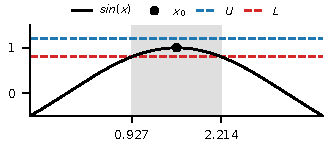
\includegraphics[width=0.32\textwidth]{figures/sine_admissible_region.pdf}
	}
	\subfloat[{Convex difference, safe zone is $[0.928, 2.203]$.}]{
	\label{sub_fig:sine_convex}
	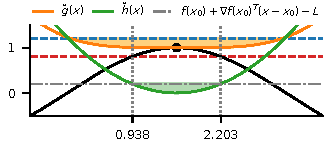
\includegraphics[width=0.32\textwidth]{figures/sine_convex_diff.pdf}
	}
	\subfloat[{Concave difference, safe zone is $[1.121, 2.202]$.}]{
	\label{sub_fig:sine_concave}
	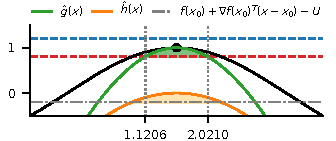
\includegraphics[width=0.32\textwidth]{figures/sine_concave_diff.pdf}
	}
	\caption{
	    ADCD local constraints for $\sin(x)$ at $x_0=\frac{\pi}{2}$.
	    Left: approximation bounds $L$ and $U$ and the resulting admissible region (gray span).
	    Middle: $\check{g},\check{h}$ of the convex difference from Lemma~\ref{lemma:adcd_by_extreme_eigenvalue}.
	    The green area shows the convex set from the upper threshold condition, and the  orange area shows the convex set of the lower threshold condition.
	    The safe zone resulting from their intersection is the area between the vertical dotted lines.
	    Right: same as middle but for $\hat{g}$ and $\hat{h}$ from the concave difference.
	}
	\label{fig:sine}
\end{figure*}




\subsection{From DC Decomposition to Constraints} 
\label{sub_sec:adcd}

After obtaining a DC decomposition of a function, the next step is to derive the ADCD local constraints.
We now show this derivation, and provide a proof that the resulting safe zone is convex, and hence guarantee correctness.

Given a convex difference $f(x) = \check{g}(x) -  \check{h}(x)$, 
we adopt the method of Lazerson et al.~\cite{lazerson:lightweight_monitoring} to derive the ADCD local constraints for $f(x)$ using the tangent plane to $\check{g}(x)$ or $\check{h}(x)$ at $x_0$:
\begin{subequations} \label{eq:convex_condition}
	\begin{align}
	&  \check{g}(x) \le \check{h}(x_0) + \nabla \check{h}(x_0)^T (x - x_0) + U, \\
	& \check{h}(x) \le \check{g}(x_0) + \nabla \check{g}(x_0)^T (x - x_0) - L.
	\end{align}
\end{subequations}
We extend this formulation for the concave difference $f(x) = \hat{g}(x) - \hat{h}(x)$, and obtain the ADCD local constraints for this difference:
\begin{subequations} \label{eq:concave_condition}
	\begin{align}
	& \hat{h}(x) \ge \hat{g}(x_0) + \nabla \hat{g}(x_0)^T (x - x_0) - U, \\
	& \hat{g}(x) \ge \hat{h}(x_0) + \nabla \hat{h}(x_0)^T (x - x_0) + L.
	\end{align}
\end{subequations}
These constraints are convex:
by opening brackets and rearranging the inequality, each inequality can be written as $\psi(x) \le C$, where $\psi$ is a convex function and $C$ is a constant, and the sets that satisfy such inequalities (sublevel sets) are convex~\cite{boyd_convex_2004}.


For the specific convex difference, in Lemma~\ref{lemma:adcd_by_extreme_eigenvalue} and in Lemma~\ref{lemma:adcd_by_eigendecomposition}, the ADCD local constraints \eqref{eq:convex_condition} can be simplified to:
\begin{align*}
\check{g}(x) \le U,\quad
\check{h}(x) \le f(x_0) + \nabla f(x_0)^T (x - x_0) - L.
\end{align*}
For the concave difference the ADCD local constraints \eqref{eq:concave_condition} are:
\begin{align*}
\hat{h}(x) \ge f(x_0) + \nabla f(x_0)^T (x - x_0) - U,\quad
\hat{g}(x) \ge L.
\end{align*}

To get the simplified form of \eqref{eq:convex_condition}, we simply note that for $\check{g},\check{h}$ in both Lemmas, $\check{h}(x_0)=0$ and $\nabla \check{h}(x_0) = 0$ and, $\check{g}(x_0) = \check{f}(x_0)$ and $\nabla \check{g}(x_0) = \nabla \check{f}(x_0)$.
Similarly, we can get the simplified form of \eqref{eq:concave_condition}.




Figure~\ref{fig:sine} shows an example of the ADCD local constraints derived for $\sin(x)$ at point $x_0=\pi/2$ according to Lemma~\ref{lemma:adcd_by_extreme_eigenvalue}.
Figure~\ref{sub_fig:sine_admissible_region} shows the admissible region, while \ref{sub_fig:sine_convex} and \ref{sub_fig:sine_concave} show the ADCD local constraints and the resulting safe zones when using convex and concave difference representations, respectively.
While both safe zones are a subset of the admissible region, they are not equivalent;
We explore this in the next subsection.




\subsection{Convex vs. Concave Difference} \label{sub_sec:convex_vs_concave_difference}

Both ADCD-X and ADCD-E provide two possible representations for a function: as a convex or as a concave difference.
In some cases, a convex difference is more efficient and results in fewer safe zone violations, while in other cases the concave difference is preferable.

Consider again the example in Figure~\ref{fig:sine} showing $\sin(x)$ with the reference point $x_0=\pi/2$.
The convex difference representation in Figure~\ref{sub_fig:sine_convex} results in a wider safe zone than the concave representation in Figure~\ref{sub_fig:sine_concave}.
Since $f$ near $x_0$ is already concave, using the concave difference results in a $\hat{g}(x)$ that is even more concave around $x_0$ than the original function $f(x)$.
However, using the convex difference obtains a convex function $\check{g}(x)$ that is "wider" than the concave function $\hat{g}(x)$, and "wider" functions tend to obtain larger safe zones.
Hence, in this case, the convex difference representation is preferable.

The curvature of $\check{g}$, $\check{h}$, $\hat{g}$, and $\hat{h}$ is determined by the eigenvalues of the Hessians of these functions, and this curvature impacts the performance of the algorithm.
Therefore, we propose the \emph{DC Heuristic} for choosing between the convex difference and concave difference, based on these eigenvalues:
if
\begin{equation*}
    \lambda_{\min} \left( H_{\check{g}}(x_0) \right) + \lambda_{\min} \left( H_{\check{h}}(x_0) \right) \le \abs{ \lambda_{\max} \left( H_{\hat{h}} (x_0) \right) + \lambda_{\max} \left( H_{\hat{g}} (x_0) \right) }
\end{equation*}
use the convex difference, otherwise use the concave difference.

The intuition behind this heuristic is to choose the representation whose two functions are less convex/concave near the reference point $x_0$.
For functions with a constant Hessian, when using ADCD-E, the heuristic condition is equivalent to $\abs{\lambda_{\min}} \le \lambda_{\max}$.

In our preliminary experiments, this heuristic reduced safe zone violations by up to 30\% when compared to using either simply the convex difference or simply the concave difference when monitoring functions such as $\sin(x)$.

\subsection{The Distributed Protocol}
\label{sub_sec:basic-protocol}

We can now describe the protocol for AutoMon coordinator and nodes, which is based on the GM protocol;
the protocol is summarized in Algorithm~\ref{algo:protocol}.
The coordinator first collects local vectors, sets $x_0 = \bar{x}$, and updates the thresholds $U$ and $L$ based on $f(x_0)$ and the desired approximation.
Next, the coordinator uses ADCD to derive correct convex local constraints in a \emph{neighborhood} $\FB$ around $x_0$.
Finally, it distributes these local constraints to all nodes.

\begin{algorithm}
	\caption{AutoMon protocol for coordinator and node.}
	\label{algo:protocol}
	\begin{algorithmic}[1]
		%
		\Procedure{CoordinatorFullSync}{} \label{step:full-sync}
		\State Pull all nodes $x^i$ and update $x_0$: $x_0 \leftarrow \frac{1}{n} \sum_{i=1}^{n} x^i$  \label{step:update-ref-point}
		\State Use $f(x_0)$ to update the thresholds $L$ and $U$
		\State Update the neighborhood $\FB$ from  $x_0$ 
		\State Compute DC decomposition of $f$
		\State Choose between convex difference and concave difference
		\State Derive safe zone based on the chosen DC
		\State Sync all nodes with the safe zone and neighborhood $\FB$
		%
		\EndProcedure

		\Procedure{NodeDataUpdate}{sample from local stream}
		\State Update the local vector $x$ using the new sample
		\If {$x \notin$ $\FB$} Report neighborhood violation and \oldReturn 
		\EndIf \label{step:neighborhood-check}
		\If {$x \notin$ safe zone} Report safe zone violation and \oldReturn
		\EndIf  \label{step:safezone-check}
		\EndProcedure		
		\Procedure{NodeUpdateConstraint}{safe zone, $\FB$}
		\State Update safe zone and the neighborhood $\FB$
		\EndProcedure
	\end{algorithmic}
\end{algorithm}

Let $\FB$ be the neighborhood of size $r$ around the reference point $x_0$: $\FB = \{ x : x \in [x_0-r,x_0+r] \}$.\footnote{In practice, we also restrict the neighborhood $\FB$ to be contained in the domain $\FD$.}
When the neighborhood is restricted, we have two types of violations.
The first type is \emph{safe zone violation}, which is caused when the node's local vector is outside the safe zone.
The second type is \emph{neighborhood violation}, which is caused when the node's local vector is outside the neighborhood of $x_0$.
The coordinator uses either type of ADCD to derive the ADCD local constraints.
For ADCD-X, it applies Lemma~\ref{lemma:adcd_by_extreme_eigenvalue} with $\FS=\FB$.
In this case, the ADCD local constraints are based on eigenvalues that are evaluated inside a specific neighborhood.
Hence, these local constraints are applicable only to this neighborhood:
they maintain correctness as long as all the local vectors are inside $\FB$.
Nodes must therefore first determine that the local vector is inside $\FB$ before checking for a safe zone violation.
Note that when using ADCD-E, the coordinator uses Lemma~\ref{lemma:adcd_by_eigendecomposition}; in this case, the neighborhood is the entire $f$'s domain $\FD$ since the Hessian is constant. 

At initialization, the coordinator first determines whether to use ADCD-X or ADCD-E, depending on the function to approximate $f$ (\S\ref{sec:adcd_by_extreme_eigenvalue} and \S\ref{sec:adcd_by_eigendecomposition}).
If ADCD-E is used, the coordinator evaluates $H^-$ and $H^+$.
If ADCD-X is used, the coordinator uses the designed approximation error bound $\epsilon$ to evaluate the optimal neighborhood size $\hat{r}$ using the tuning algorithm presented in the next section.


The node algorithm is simple: whenever there is an update to the local vector, the node will check if the data remains in the neighborhood $\FB$ and whether the ADCD local constraints still hold.
If not, the node will report a violation to the coordinator.
Otherwise, the node does nothing.
Whenever an updated local constraint arrives from the coordinator, it will use the new constraint.


\betterparagraph{Lazy Sync and Slack}
We incorporate two commonly-used enhancements to the above protocol, which help reduce the number of local violations and allow the coordinator to resolve them without pulling local vectors from all the nodes.
As they are not the focus of this work, we only include necessary detail, and refer the reader to prior work~\cite[Sec.~4.2 and~4.6]{gabel:entropy_approximation} for description and analysis.

With \emph{slack}, nodes add a \emph{slack vector} $s^i$ to the local vector $x^i$ when checking the local constraints (Alg.~\ref{algo:protocol}, lines~\ref{step:neighborhood-check} and~\ref{step:safezone-check});
$s^i$ is set by the coordinator to $x_0 - x^i$ whenever we update $x_0$ (line~\ref{step:update-ref-point}).
%
\emph{Lazy sync} is an incremental approach to resolving safe zone violations.
When a violation is reported to the coordinator, it starts adding nodes one by one to a \emph{balancing set} $\FS$ until either the violation is resolved (in which case it rebalances $s^i$ for the nodes in $\FS$ and monitoring resumes without changing $x_0$), or until $\vert \FS \vert > \frac{n}{2}$ (in which case it falls back to the full sync in line~\ref{step:full-sync}).
We use a least-recently used (LRU) strategy to select nodes to add to $\FS$.
%
We explore the impact of slack and lazy sync in \S\ref{sub_sec:rlv_and_lazy_sync}.

\subsection{Setting the Neighborhood Size} 
\label{sub_sec:sub_domain_size}


ADCD-X requires finding the extreme eigenvalues in a neighborhood $\FB$ of size $r$ around $x_0$.
The choice of neighborhood size $r$ is important since it affects the eventual efficiency of the ADCD local constraints.
An increase in $r$ leads to increase in the search domain for $\lambda_{\min}$ and $\lambda_{\max}$, which can results in more extreme eigenvalues than a smaller $r$ produces, resulting in different DC decomposition.

Interestingly, while prior work observed that different constraints are optimal in different regions of the data space~\cite{lazerson:lightweight_monitoring}, the question of neighborhood size did not come up.
Prior work focused on 
finding analytically-derived constraints designed to be \emph{globally correct}: correct everywhere in $f$'s domain $\FD$.
In contrast, ADCD provides a neighborhood around the reference point, which in turn means the ADCD local constraints need only be correct for data inside the neighborhood $\FB$.
Hence, ADCD constraints are \emph{locally correct}.

\begin{figure}
	\centering
	\subfloat[Smaller neighborhood.]{
	\label{sub_fig:domain_sz_tradeoff_small_domain}
    \quad	
	\scalebox{0.5}{\pagestyle{empty}

\definecolor{ffqqqq}{rgb}{1,0,0}
\definecolor{wrwrwr}{rgb}{0.3803921568627451,0.3803921568627451,0.3803921568627451}
\definecolor{rvwvcq}{rgb}{0.08235294117647059,0.396078431372549,0.7529411764705882}

\begin{tikzpicture}[line cap=round,line join=round,>=triangle 45,x=1cm,y=1cm,yscale=0.8]
\tikzstyle{every node}=[font=\huge]
\begin{scope}
  \clip (-1.2,-0.5) circle (1.441395932235966cm);
  \fill[rvwvcq!20] (-2.4,-1) rectangle (-0.6,1);
\end{scope}
\draw [line width= 1pt,color=wrwrwr] (-1.2,-0.5) circle (1.441395932235966cm);
\draw[line width=1pt,color=black, dashed] (-2.4,-1) rectangle (-0.6,1);

\draw[thick, smooth, color=ffqqqq] plot coordinates
{
	(-3.5,1.3)
	(-3.2,2.2)
	(-0.1,1.8)
	(0.4,0)
	(0.8,-0.6)
	(0.6,-1.2)
	(-0.4,-1.8)
	(-2,-2.4)
	(-2.7,-1.6)
	(-3.7,-0.8)
	(-3.3,0.5)
	(-3.5,1.3)
};

\begin{scriptsize}
\node [fill=black, circle, inner sep=1.5pt, outer sep=1pt, label=above:$x_0$] (x0) at (-1.5,0) {};
\draw [color=black] (-2.513809523809525,1.5) node {$\FB$};
\draw (-1.2,-1.32) node {safe zone};
\draw [color=ffqqqq] (0.15,1.99) node {$\FA$};
\end{scriptsize}
\end{tikzpicture}
}
	\quad
	}
	\qquad
	\subfloat[Larger neighborhood.]{
    \quad	
	\label{sub_fig:domain_sz_tradeoff_large_domain}
	\scalebox{0.5}{\pagestyle{empty}

\definecolor{ffqqqq}{rgb}{1,0,0}
\definecolor{wrwrwr}{rgb}{0.3803921568627451,0.3803921568627451,0.3803921568627451}
\definecolor{rvwvcq}{rgb}{0.08235294117647059,0.396078431372549,0.7529411764705882}

\begin{tikzpicture}[line cap=round,line join=round,>=triangle 45,x=1cm,y=1cm, yscale=0.8]
\tikzstyle{every node}=[font=\huge]
\draw [line width=1pt,color=wrwrwr, fill=rvwvcq!20] (-1.5561710992112803,-0.06440353297281982) circle (0.8580930430876647cm);
\draw[line width=1pt,color=black,dashed] (-4.0,-2.5) rectangle (1.0,2.5);

\draw[thick, smooth, color=ffqqqq] plot coordinates
{
	(-3.5,1.3)
	(-3.2,2.2)
	(-0.1,1.8)
	(0.4,0)
	(0.8,-0.6)
	(0.6,-1.2)
	(-0.4,-1.8)
	(-2,-2.4)
	(-2.7,-1.6)
	(-3.7,-0.8)
	(-3.3,0.5)
	(-3.5,1.3)
};
			
\begin{scriptsize}
\node [fill=black, circle, inner sep=1.5pt, outer sep=1pt, label=above:$x_0$] (x0) at (-1.5,0) {};
\draw [color=black] (-4.35,2.2) node {$\FB$};
\draw (-1.30272727272727273,-1.4) node {safe zone};
\draw [color=ffqqqq] (0.1,2.0) node {$\FA$};
\end{scriptsize}
\end{tikzpicture}
}
    \quad	
	}
	\caption{
		Tradeoff between neighborhood size (dashed rectangle) and the resulting safe zone size (solid circle). 
		The local constraint is their intersection (shaded area).
	}
	\label{fig:domain_sz_tradeoff}
\end{figure}

This presents us with a new opportunity: since ADCD constraints need only be locally correct, they can be more permissive, resulting in fewer safe zone violations.
The challenge lies in balancing the tradeoff between neighborhood and safe zone violations.
%
If the neighborhood $\FB$ is very small (small $r$), the resulting safe zone can be large, but local data easily moves outside the neighborhood, which means more \emph{neighborhood violations (i.e., $x \notin \FB$)}.
If $\FB$ is very large (large $r$) there will be few neighborhood violations, but the resulting safe zone might be needlessly restrictive due to more extreme eigenvalues, resulting in many safe zone violations.
%
Figure~\ref{fig:domain_sz_tradeoff} illustrates this tradeoff.
In Figure~\ref{sub_fig:domain_sz_tradeoff_small_domain} the neighborhood $\FB$ is very small, resulting in a large safe zone but potentially many neighborhood violations.
In Figure~\ref{sub_fig:domain_sz_tradeoff_large_domain} $\FB$ is very large and in fact $\FB$ is a super-set of the admissible region $\FA$ and hence there can be no neighborhood violations.
However, this also results in a much smaller safe zone which could lead to many safe zone violations.




\betterparagraph{Effect of Neighborhood Size $r$}
To explore the impact of the neighborhood size on the number of violations, we used AutoMon to monitor the Rozenbrock function $f(x) = (1 - x_1)^2 + 100 \left(x_2 - x_1^2\right)^2$, where $x_1,x_2$ are sampled from the normal distribution $\mathcal{N}(0, 0.2^2)$.
We used additive approximation with approximation error bound $\epsilon$: $L = f(x_0) - \epsilon, U = f(x_0) + \epsilon$.
For a given approximation error bound $\epsilon$ we monitor the function with different values of $r$, and count the total number of neighborhood and safe-zone violations.

\begin{figure}
	\centering
	{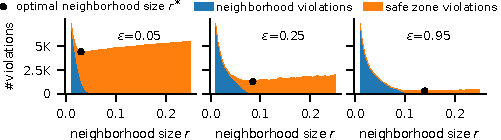
\includegraphics[width=1.0\columnwidth]{figures/impact_of_neighborhood_on_violations_three_error_bounds.pdf}}
	\caption{
	    The effect of neighborhood size $r$ on the number of violations while monitoring Rozenbrock function with four different approximation error bounds.
	}
	\label{fig:impact_of_neighborhood_on_violations_three_error_bounds}
\end{figure}


Figure~\ref{fig:impact_of_neighborhood_on_violations_three_error_bounds} shows the number of violations as a function of neighborhood size for four different approximation error bounds $\epsilon \in \{0.05, 0.25, 0.95\}$.
For a specific $\epsilon$, we observe the tradeoff
between neighborhood violations and safe zone violations.
Additionally, we see that permissive approximation error bounds (larger $\epsilon$) imply larger safe zones, resulting in fewer safe zone violations.
Increasing $\epsilon$ results in slightly more neighborhood violations, which we discuss below.
Lastly, we observe that neighborhood violations decrease when the neighborhood size increases, as expected.



Safe zone and neighborhood violation can hide each other.
Since the nodes check for neighborhood violation before checking the ADCD local constraint, some of the safe zone violations are concealed by neighborhood violations.
However, the opposite also happens.
When $\epsilon$ is small, the resulting small safe zone leads to many safe zone violations. 
When these are resolved, the coordinator updates $x_0$ and the neighborhood $\FB$, meaning that a future neighborhood violations are less likely. 
Therefore smaller $\epsilon$ results in fewer neighborhood violations.

\begin{algorithm}[t]
	\caption{Neighborhood Size Tuning}
	\begin{algorithmic}
		%
		\State $b \gets 1$
		\State \textbf{while} NoNeighborhoodViol(monitor with $r=b$) \textbf{do} $b \gets b / 2$
		\State $lo \gets b$, $hi \gets b$
		\State \textbf{while} AnySafezoneViol(monitor with $r=lo$) \textbf{do} $lo \gets lo / 2$
		\State \textbf{while} AnyNeighborhoodViol(monitor with $r=hi$) \textbf{do} $hi \gets 2\cdot hi$
		\State $R \gets 10$ equally spaced $r$ values in the range $[lo, hi]$
		\Return $\operatorname{argmin}_{r' \in R}$ NumTotalViolations(monitor with $r=r'$)
	\end{algorithmic}
	\label{algo:sub_domain_tuning}
\end{algorithm}



\betterparagraph{Tuning Procedure}
The optimal neighborhood size $r^*$, shown in Figure~\ref{fig:impact_of_neighborhood_on_violations_three_error_bounds} as a dot, is the neighborhood size that obtains the smallest number of violations in total.
The optimal size $r^*$ depends on the function, the data, and the allowed approximation error $\epsilon$.

To avoid the user needing to specify the neighborhood size $r$, AutoMon automatically tunes for the approximated optimal size $\hat{r}$.
This is done by running AutoMon on a small subset of the initial data and counting violations.
Algorithm~\ref{algo:sub_domain_tuning} is the tuning algorithm to find the approximated optimal neighborhood size $\hat{r}$.
It finds a low neighborhood size $r$ for which there are no safe zone violation and a high $r$ with no neighborhood violations, and then returns a neighborhood size in between with fewest total violations.
We evaluate the effectiveness of this tuning procedure in \S\ref{sec:eval-sub-domain-size}.

Since tuning is done on a small subset of the data, later changes in data distribution can mean $\hat{r}$ found by the tuning process becomes too small, causing unnecessary neighborhood violations.
In our experience this is rare, mostly when the error bound is very large.
We mitigate this using a simple heuristic:
whenever the coordinator observes $5 n$ consecutive neighborhood violations with no intervening safe zone violations, it multiplies $\hat{r}$ by 2.
We leave adaptive tuning of $r$ to future work.




\subsection{Assumptions and Correctness Guarantees}
\label{sec:correctness_guarantees}

AutoMon's correctness guarantees are given under three core assumptions.
First, we make the mild assumption that automatic differentiating obtains accurate Hessians.
Second, we assume nodes and coordinator communicate using an underlying messaging fabric which guarantees delivery.
Third, we assume that the rate in which each node receives local data is lower than the maximum time to resolve violations, which depends on the network latency and the time it takes the coordinator to compute local constraints.

Under these assumptions,
AutoMon provides a deterministic correctness guarantee if the representation used to derive the ADCD local constraints is a true DC decomposition in $\FB$, i.e. $\check{g} , \check{h}$ are convex or $\hat{g}, \hat{h}$ are concave in $\FB$.
In this case, the local constraints are convex (\S\ref{sub_sec:adcd}).
This convexity implies that if all local vectors $x^i$ are within AutoMon's safe zone, then any convex combination of $x^i$, including $\bar{x}=\frac{1}{n}\sum x^i$, is inside the safe zone, thus $L \le f(\bar{x}) \le U$.

Therefore, ADCD provides strong correctness guarantee when approximating functions with constant Hessian, as ADCD-E obtains true DC decomposition.
%
In addition, ADCD-X provides correctness guarantee when approximating convex and concave functions.
For any convex function the minimal eigenvalue of $H(x)$ at every $x \in \FD$ is non-negative.
Hence $\hat{\lambda}$ found by the optimization process is non-negative and $\lambda^-_{\min}=0$.
Since $0 \le \lambda^+_{\max}$, the DC Heuristic chooses the convex difference, which is a true DC decomposition as $\lambda^-_{\min}$ is a lower bound for $\lambda_{\min}$.

ADCD-X does not necessarily guarantee correctness for other arbitrary functions since the optimization problem \eqref{eq:numerical_eigenvalues} may converge on a local solution; inaccurate $\lambda^-_{\min}$ and $\lambda^+_{\max}$ values can result in representation that is not a DC decomposition.
%
We mitigate this using a simple sanity check.
Recall that by construction, AutoMon's safe zone defined by the local constraints is included in the admissible region.
Thus, whenever the local vector $x$ is inside the safe zone, nodes also verify that $L \leq f(x) \leq U$ (i.e., $x \in \FA$).
%
In the rare case where this verification fails, the node notifies the coordinator about a violation and indicates that the local constraints are faulty;
the coordinator then initiates a full sync.
%
Our evaluation shows AutoMon provides a good approximation for even highly non-convex functions with discontinuous derivatives
such as neural networks with ReLU activations (\S\ref{sec:evaluation}).


\subsection{Library API} 
\label{sec:implementation}

AutoMon is not a complete distributed data processing system.
Like sketches (\S\ref{sec:related_work}), AutoMon is an algorithmic building block for building such systems (potentially using existing software frameworks~\cite{flink}).
We therefore design AutoMon as an agnostic library that focuses strictly on the monitoring algorithm.
Application details and system-level support for reading data, messaging, deployment, and so on are outside the scope of this library, and are the responsibility of the user.
In particular, the developer must mediate between AutoMon and a messaging fabric of their choice:
the developer uses the library API to produce or consume message contents, which the messaging fabric transfers over the network.\footnotemark{}
\footnotetext{We provide an example of a ZeroMQ~\cite{zeromq} mediation layer in AutoMon's code repo.}


Given a function presented as a numeric program in a high-level language, AutoMon provides the basic API required to perform distributed monitoring of the function.
The user first initializes an AutoMon node, \lstinline[frame=no]{node = AutoMonNode(f, epsilon)}, passing the function to monitor and the required approximation.
Retrieving the current approximated value of the function is simply a matter of calling the \lstinline{node.current_value()} method which returns $f(x_0)$.  
%
The user must notify AutoMon when the local vector $x$ has changed by calling \lstinline{node.update_data(x)}, and send any resulting message (e.g., safe zone violation) to the coordinator;
AutoMon will provide and process the contents of such messages.
Similarly, when a message has been received from the coordinator the user must call \lstinline{node.message_received(msg)}, then send back any reply.
